% !TEX program = xelatex
\documentclass[tikz, crop, border = {2pt 2pt 2pt 2pt}]{standalone}

\usepackage{concmath-otf}
\usetikzlibrary{calc, angles, quotes, patterns, decorations.pathreplacing, decorations.pathmorphing, calligraphy, arrows.meta}

\begin{document}
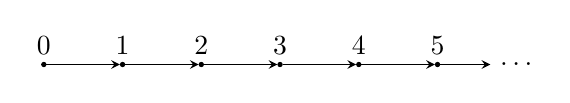
\begin{tikzpicture}
	\tikzstyle {pointlike} = [draw, fill = black, circle, inner sep = 0pt, minimum size = 1.5pt];
	\foreach \nodename in {0, 1, 2, ..., 5} {
			\node[pointlike] (\nodename) at (\nodename, 0) {} node[above] at (\nodename) {\(\nodename\)};
		}
	\node (6) at (6, 0){\(\dots\)};
	\foreach \firstnode/\secondnode in {0/1, 1/2, 2/3, 3/4, 4/5, 5/6} {
			\draw[-stealth] (\firstnode) -- (\secondnode);
		}
\end{tikzpicture}
\end{document}







